\documentclass[12pt,fullpage,letterpaper]{article}

\newenvironment{proof}{\noindent{\bf Proof:}}{\qed\bigskip}

\newtheorem{theorem}{Theorem}
\newtheorem{corollary}{Corollary}
\newtheorem{lemma}{Lemma}
\newtheorem{claim}{Claim}
\newtheorem{fact}{Fact}
\newtheorem{definition}{Definition}
\newtheorem{assumption}{Assumption}
\newtheorem{observation}{Observation}
\newtheorem{example}{Example}
\newcommand{\qed}{\rule{7pt}{7pt}}

\newcommand{\assignment}[4]{
\thispagestyle{plain}
\newpage
\setcounter{page}{1}
\noindent
\begin{center}
\framebox{ \vbox{ \hbox to 6.28in
{\bf CS446: Machine Learning \hfill #1}
\vspace{4mm}
\hbox to 6.28in
{\hspace{2.5in}\large\mbox{Problem Set #2}}
\vspace{4mm}
\hbox to 6.28in
{{\it Handed Out: #3 \hfill Due: #4}}
}}
\end{center}
}


\newcommand{\handout}[3]{
\thispagestyle{plain}
\newpage
\setcounter{page}{1}
\noindent
\begin{center}
\framebox{ \vbox{ \hbox to 6.28in
{\bf CS446: Machine Learning \hfill #1}
\vspace{4mm}
\hbox to 6.28in
{\hspace{2.5in}\large\mbox{#2}}
\vspace{4mm}
\hbox to 6.28in
{{\it Handed Out: #3 \hfill }}%Name (NetID): \rule[-2pt]{4cm}{0.1pt} }}
}}
\end{center}
}


\newcommand{\assgsoln}[4]{
\thispagestyle{plain}
\newpage
\setcounter{page}{1}
\noindent
\begin{center}
\framebox{ \vbox{ \hbox to 6.28in
{\bf CS446: Machine Learning \hfill #1}
\vspace{4mm}
\hbox to 6.28in
{\hspace{2.5in}\large\mbox{Problem Set #2 Solutions}}
\vspace{4mm}
\hbox to 6.28in
{{\it Handed Out: #3 \hfill Handed In: #4}}
}}
\end{center}
}


\newcommand{\solution}[4]{
\thispagestyle{plain}
\newpage
\setcounter{page}{1}
\noindent
\begin{center}
\framebox{ \vbox{ \hbox to 6.28in
{\bf CS446: Machine Learning \hfill #4}
\vspace{4mm}
\hbox to 6.28in
{\hspace{2.5in}\large\mbox{Problem Set #3}}
\vspace{4mm}
\hbox to 6.28in
{#1 \hfill {\it Handed In: #2}}
}}
\end{center}
\markright{#1}
}


\newenvironment{algorithm}
{\begin{center}
\begin{tabular}{|l|}
\hline
\begin{minipage}{1in}
\begin{tabbing}
\quad\=\qquad\=\qquad\=\qquad\=\qquad\=\qquad\=\qquad\=\kill}
{\end{tabbing}
\end{minipage} \\
\hline
\end{tabular}
\end{center}}

\def\Comment#1{\textsf{\textsl{$\langle\!\langle$#1\/$\rangle\!\rangle$}}}



\oddsidemargin 0in
\evensidemargin 0in
\textwidth 6.5in
\topmargin -0.5in
\textheight 9.0in

% \renewcommand\thesection{\alpha{section}} 
\usepackage{csquotes}
\usepackage{amsmath}
\usepackage[colorlinks]{hyperref}
\usepackage{graphicx}
\graphicspath{{images/}}

\begin{document}

\solution{Kexin Hui}{\today}{1}{Spring 2017}
% Fill in the above, for example, as follows:
% \solution{Joe Smith}{\today}{1}{Fall 2012}

\pagestyle{myheadings}  % Leave this command alone

\begin{enumerate}
\item Answer to problem 1 - Learning Conjunctions

	\begin{enumerate}\parindent -4pt
	
	\item [a.]
	My algorithm is to first propose a most general hypothesis based on a randomly picked positive labeled instance. Then rule out the inconsistences when iterating through all other positive training examples. Here, inconsistence occurs when one of the elements does not comply with the proposed hypothesis. Once we finish with the iteration through positive training data, we will do the final check using all training examples to see if there exists a negative example completely consistent with our proposed hypothesis or there exists a positive example inconsistent with our hypothsis.

	\noindent\rule[0.5ex]{\linewidth}{1pt}
	1.    Get \emph{m} training instances of Boolean vectors of size \emph{n}; \\
	2.    Given one $positive$ labeled instance $(1, 0, 1, 0, 0, 0, 1, ..., 0)$;\\
	3.    Assume $hypothesis  =\ (x_{1} = 1 \land x_{2} = 0 \land x_{3} = 1 \land x_{4} = 0 \land ... \land x_{n}=0)$; \\
	4.    For each $positive$ instance \emph{x}: \\
	5.   \qquad For \emph{i} from 1 to \emph{n}: \\
	6.   \qquad \qquad If $x_i$ is not consistent with $hypothesis$: \\
	7.   \qquad \qquad \qquad Remove $x_i$ term from $hypothesis$; \\
	8.    If $hypothesis$ is empy: \\
	9.   \qquad Return \enquote{$no\> consistent\> hypothesis$}; \\
	10. For each  instance $x$: \\
	11. \qquad If $x$ is labeled $negative$: \\
	12. \qquad \qquad If all $n$ items of $x$ are consistent with $hypothesis$ :\\
	13. \qquad \qquad \qquad Return \enquote{$no\> consistent\> hypothesis$}; \\
	14. \qquad If $x$ is labeled $positive$: \\
	15. \qquad \qquad If any one of the $n$ items is inconsistent with $hypothesis$:\\
	16. \qquad \qquad \qquad Return \enquote{$no\> consistent\> hypothesis$}; \\
	17. Return $hypothesis$; \\
	\noindent\rule[0.5ex]{\linewidth}{1pt}

	\item[b.]
	I believe the algorithm is correct since a final consistency check through all training instances is done after the first iteration through all positive training data to decide the result hypothesis. On the other hand, conjunction means that the instance should satisfy all of the condition terms of the hypothesis in order to be determined as positive. A hypothesis is proposed at first based on a random positive instance we are given. Then when we loop through all the positive examples to eliminate the inconsistence between the current hypothesis and training data. For example, the current hypothesis is ($x_1 = 1 \land x_2 = 0 \land x_4 = 0 \land x_5 = 1 \land ... $), and the current positive training example is ($ x_1 =1 \land x_2 = 1 \land x_3 = 1 \land x_4 = 1 \land x_5 = 1 \land ... $). Clearly, we can see that $x_1$  and $x_5$ terms are consistent, while $x_2$ and $x_4$ terms are inconsistent. Again, because it is a conjunction hypothesis, $x_2$ and $x_4$ could not be in the hypothesis and would be ruled out. Therefore, all consistent terms are preserved in order to generate the result hypothesis. 
	
	There is also another way to think about the correctness of my algorithm. If the algorithm does output a hypothesis, the hypothesis should be consistent since it passes through all the positive training data and also the second-round check in the. If the algorithm outputs no consistent hypothesis, it could possibly because the input is not consistent itself by human errors. Or there are not sufficient enough positive training examples for us to determine a most general hypothesis.
	
	\item[c.]
	The initialization of the vector space of $n$ training data is $O(n)$. Proposing a initialized hypothesis is $O(1)$. During the first iteration of all positive training data, we check each dimension of the Boolean vector to rule out the inconsistency, which would make $O(mn)$ time. In the second consistency check of all $n$ training data, again it takes $O(mn)$.  Thus, the running time should be $O(mn)$.
	
	\item[d.]
	The hypothesis derived by the algorithm above could be quite accurate. If the algorithm determines the test example to be positive, it must be positive since this is what we can tell based on what training data we are given. However, if the algorithm determines the test example to be negative, it might not be the case. The reason is that the hypothesis we proposed might not be the most general case given the limited training data. The way we generate a hypothesis is to always find the intersection between the current hypothesis and the positive training data. In other words, false positive may occur. 
	
	\end{enumerate}

\item Answer to problem 2 - Linear Algebra Review

	\begin{enumerate}\parindent -4pt
	
	\item[a.]
	As an extension from 2-dimensional hyperplane that we are familiar with, we can always find a normal vector $\vec{n}$, which is perpendicular to all vectors in the given hyperplane $\vec{\omega}^T \vec{x}+\theta =  0 $. That is, $\vec{n} \perp \vec{x}$, $\forall \vec{x} \in \left \{ \vec{x} \>|\> \vec{\omega}^T \vec{x}+\theta =  0 \right \}$. Similar to what we do in 2D hyperplane, the distance $d$ between the particular point $\vec{x}_0$ and the hyperplane is the projection of $\vec{x}-\vec{x}_0$ onto $\vec{n}$, where $\vec{x}$ is any arbitrary point in this hyperplane. The equation of the distance is given by:
	\begin{equation*}
	d = \frac{\left | \vec{n}\cdot \vec{x} \right |}{\left \| \vec{n}\right \|} = \frac{\left | \vec{\omega}^T \vec{x}_0 + \theta \right |}{\left \| \vec{\omega} \right \|}
	\end{equation*}
	
	\item[b.]
	After a close scrutiny of the hyperplane function $\vec{\omega}^T \vec{x}+\theta =  0 $, $\theta$ can be sort of viewed as an intercept and $\vec{\omega}^T$ as the slope by analogy to 2-dimensional hyperplane. Therefore, we can think of the two hyperplanes we are given as two parallel hyperplanes with the same slope but different intercepts. Since they are parallel to each other, the distance denoted by $d$ between these two hyperplanes is quite straightforward, given by:
	\begin{equation*}
	d = \frac{\left | \theta_1 - \theta_2 \right |}{\left \| \vec{\omega} \right \|}
	\end{equation*}
	
	\end{enumerate}

\item Answer to problem 3 - Finding a Linear Discriminant Function via Linear Programming

	\begin{enumerate} \parindent -4pt
	
	\item[a.1]
	In order to show that D is linearly separable if and only if there exists a hyperplane that satisfies the linear program condition with $\delta = 0$, we need to show the relationship in both directions. 
	
	\medskip
	On one hand, $\delta = 0 \Rightarrow Linear\> Separability$. \\
	Suppose there exists a hyperplane that satisfies the condition that 
	\begin{equation*}
	y_i(\vec{\omega}^T\vec{x}_i + \theta) \geq 1, \forall(\vec{x}_i,y_i)\in D 
	\end{equation*}
	Therefore, it is quite straightforward to conclude from the equation that
	\begin{equation*}
	when\> y_i = 1,\>\> \vec{\omega}^T\vec{x}_i + \theta \geq 1 \geq 0
	\end{equation*}
	\begin{equation*}
	when\> y_i = -1, \>\vec{\omega}^T\vec{x}_i + \theta \leq -1 <0
	\end{equation*}
	It is obvious then the hyperplane is linearly separable. 
	
	\medskip
	On the other hand, $Linear\>Separability \Rightarrow \delta = 0$. \\
	Suppose there are two examples closest to the hyperplane $\vec{\omega}^T\vec{x}_i + \theta$, let $\vec{p}$ denote the closest positive example to the hyperplane, and $\vec{n}$ denote the closest negative example. And these two examples satisfy the linear separability as shown below,
	\begin{equation*}
	y^+ = 1, \>\>\>\vec{\omega}^T\vec{p}+ \theta =  \min(\vec{\omega}^T\vec{x}_i + \theta) \geq 0, \>\forall(\vec{x}_i,y_i)\in D
	\end{equation*}
	\begin{equation*}
	y^- = -1, \>\vec{\omega}^T\vec{n}+ \theta = \max(\vec{\omega}^T\vec{x}_i + \theta) < 0, \>\forall(\vec{x}_i,y_i)\in D
	\end{equation*}
	Note that two distances from each example to the hyperplane may be different. We could always shift the hyperplane a little bit to a position where the distance from the two closest point of each side to the hyperplane is the same. Then the new distance becomes $\frac{\min(\vec{\omega'}^T\vec{p} + \theta') - \max(\vec{\omega'}^T\vec{n} + \theta')}{2}$ for both the closest positive and negative example, which is also the minimum distance for all data to the separable hyperplane. $y_i$ can be viewed as a multiplier to ensure the result is always positive. Therefore, after shifting the hyperplane, we get
	\begin{equation*}
	y_i(\vec{\omega'}^T\vec{x}_i + \theta') \geq \frac{\min(\vec{\omega'}^T\vec{p} + \theta') - \max(\vec{\omega'}^T\vec{n} + \theta')}{2}
	\end{equation*} 
	Next, we can multiply a scale factor $\alpha$ at both side to make $\alpha \times \frac{\min(\vec{\omega'}^T\vec{p} + \theta') - \max(\vec{\omega'}^T\vec{n} + \theta')}{2} = 1$. It is worth mentioning that $\alpha \times (\vec{\omega'}^T\vec{x}_i + \theta')$ is the same hyperplane as $\vec{\omega'}^T\vec{x}_i + \theta'$. The inequality relationship finally becomes:
	\begin{equation*}
	y_i\times \alpha \times(\vec{\omega'}^T\vec{x}_i + \theta') \geq 1
	\end{equation*}
	\begin{equation*}
	\Rightarrow y_i(\vec{\omega}^T\vec{x}_i + \theta) \geq 1
	\end{equation*}
	Here, $\vec{\omega}$ and $\theta$ are not the same as the initial notation, but we use it for ease of reading. Clearly, the formulation holds when $\delta = 0$. 
	
	\medskip
	When $\delta > 0 $, the larger it is , the closer the distance between the hyperplane and the closest point. Yet if $\delta \geq 1$, $\vec{\omega}^T\vec{x}_i + \theta$ is greater than or equal to a negative value. Then the dataset might not be separable. 
	
	\item[a.2]
	When $\delta$ takes the minimum number as 0, the trivial solution could only be $\vec{\omega} = \vec{0}$ and $\theta = 0$. It is optimal since $\delta$ can take the smallest value and still make the inequality holds. Yet when $\vec{\omega} = \vec{0}$ and $\theta = 0$, there is actually no hyperplane, which makes nonsense. 
	
	\item[a.3]
	Plug in $\vec{x}_1, y_1 ,\vec{x}_2, y_2$ into the given formulation:
	\begin{equation*}
	\begin{split}
	y_1(\vec{\omega}^T\vec{x}_1+\theta)\geq 1-\delta \Rightarrow (\omega_1 + \omega_2 + ... + \omega_n + \theta) \geq 1-\delta \\ 
	y_2(\vec{\omega}^T\vec{x}_2+\theta)\geq 1-\delta \Rightarrow -(-\omega_1 - \omega_2 - ... - \omega_n + \theta) \geq 1-\delta
	\end{split}
	\end{equation*}
	It can also be interpreted as $\omega_1 + \omega_2 + ... + \omega_n \pm \theta \geq 1-\delta$. As a result, if we minimize $\delta$ to 0, we find the optimal solution to be:
	\begin{equation*}
	\begin{split}
	\omega_1 + \omega_2 + ... + \omega_n \geq 1\\
	\theta = 0
	\end{split}
	\end{equation*}
	
	\item[b.1]
	The purpose of this linear program problem is to find the minimum $\delta \geq 0$ that satisfies $y_i(\vec{\omega}^T\vec{x}_i + \theta) \geq 1-\delta$, where $\vec{\omega}$, $\theta$ and $\delta$ are unknown. Therefore, the parameter $\vec{t}$ we are looking for  in this problem is $[\vec{\omega}, \theta, \delta]^T$. And objective function should be $z(\vec{t}) = \vec{c}^T\vec{t} = \theta$, where the cost vector $\vec{c} = [0, 0, 0, ... , 0, 1]^T$ of n+2 dimensions. The constraint function could be changed to 
	\begin{equation*}
	\begin{split}
	y_i(\vec{\omega}^T\vec{x}_i + \theta) + \delta \geq 1\\
	\Rightarrow y_i\vec{x}_i^T\vec{\omega} + y_i\theta + \delta \geq 1
	\end{split}
	\end{equation*}
	and
	\begin{equation*}
	\delta \geq 0
	\end{equation*}
	Thus, $A =
	\begin{bmatrix}
	y_1\vec{x}_1^T & y_1     & 1        \\
	y_2\vec{x}_2^T & y_2     & 1        \\
	\vdots                & \vdots & \vdots \\
	y_n\vec{x}_n^T & y_n     & 1         \\
	0                        & 0        & 1         \\
	\end{bmatrix}$,
	$b = [1, 1, 1, ... , 1, 0]^T$ of m+1 dimensions. \\
	
	A code snippet for $findLinearDiscriminant.m$ is shown below. \\
	\noindent\rule[0.5ex]{\linewidth}{1pt}
	1.	function [w,theta,delta] = findLinearDiscriminant(data)\\
	2.	{\color{blue} \%\% setup linear program} \\
	3.	$[m, np1]$ = size(data);\\
	4.	n = np1-1;\\
	\newline
	5.	{\color{blue} \% write your code here}\\
	6.	x = data(:,1:n);\\
	7.	y = data(:,n+1);\\
	\newline
	8.	c = zeros(n+2,1);\\
	9.	c(n+2) = 1;\\
	\newline
	10.	b = ones(m+1,1);\\
	11.	b(m+1) = 0;\\
	\newline
	12.	A = zeros(m+1,n+2);\\
	13.	for i = 1:m\\
    	14.	\qquad A(i,n+1) = y(i);\\
    	15.	\qquad A(i,n+2) = 1;\\
    	16.	\qquad A(i, 1:n) = y(i) * x(i, 1:n);\\
	17.	end\\
	18.	A(m+1,n+2) = 1;\\
	\newline
	19.	{\color{blue}\%\% solve the linear program}\\
	20.	{\color{blue}\% adjust for matlab input: A*x <= b}\\
	21.	$[t, z]$ = linprog(c, -A, -b);\\
	\newline
	22.	{\color{blue}\%\% obtain w,theta,delta from t vector}\\
	23.	w = t(1:n);\\
	24.	theta = t(n+1);\\
	25.	delta = t(n+2);\\
	\newline
	26.	end\\
	\noindent\rule[0.5ex]{\linewidth}{1pt}
	
	\item[b.2]
	I manually generate a dataset that represents a monotone 2-variable conjunction, $x_1 \land x_2$, is shown below.
	\begin{center}
	\noindent\rule[0.5ex]{\linewidth}{1pt}	
	0\hspace{6pt}0\hspace{8pt}-1\\
	0\hspace{6pt}1\hspace{8pt}-1\\
	1\hspace{6pt}0\hspace{8pt}-1\\
	1\hspace{6pt}1\hspace{10pt}1\\
	\noindent\rule[0.5ex]{\linewidth}{1pt}
	\end{center}
	A code snippet for $plost2dSeparator.m$ is given below. \\
	\noindent\rule[0.5ex]{\linewidth}{1pt}
	1.  function plot2dSeparator(w, theta)\\
    	2.  \qquad x = linspace(-2,2,100);\\
    	3.  \qquad y = -w(1)/w(2)*x - theta/w(2);\\
    	4.  \qquad plot(x,y);\\
	5.  end\\
	\noindent\rule[0.5ex]{\linewidth}{1pt}
	The linear separator found by the code is:
	\begin{equation*}
	156.2452x_1 + 156.2452x_2 - 237.6709 = 0
	\end{equation*}
	And the plot for labeled data points and the corresponding linear separator is shown in the next page. \\
	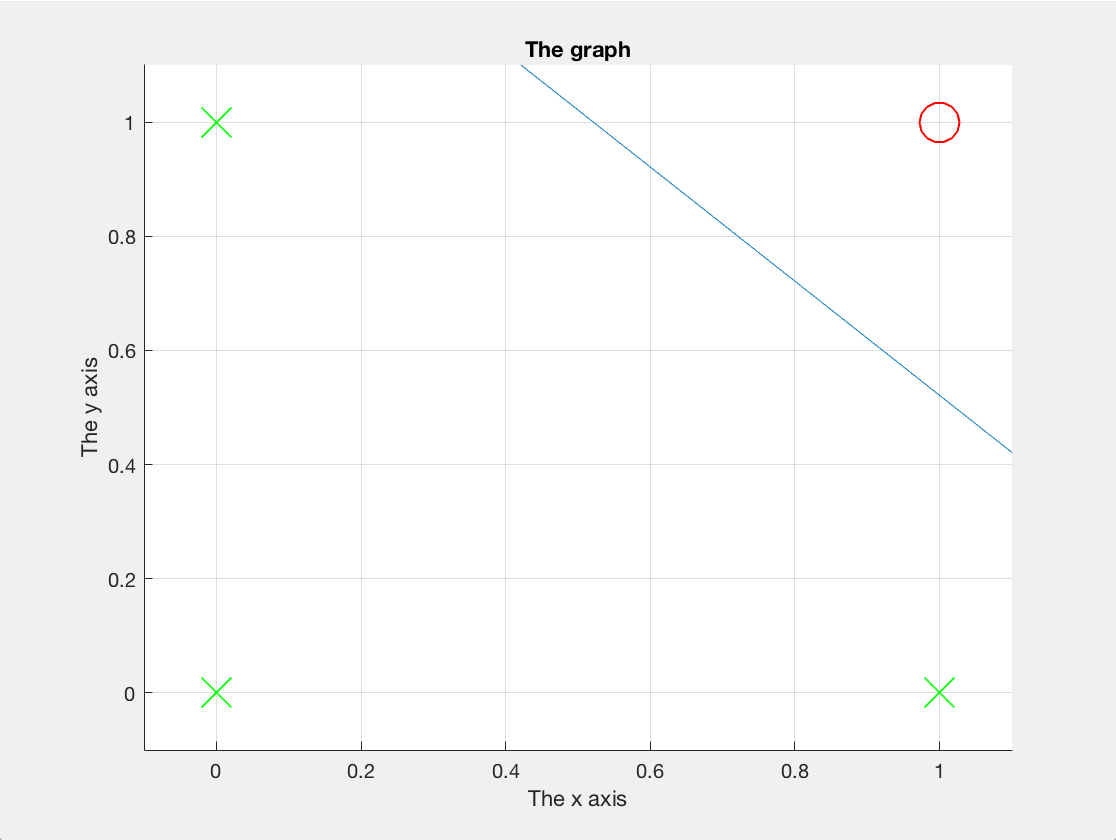
\includegraphics[scale = 0.7]{p3b2}
	After taking the data from $hw1conjunctions.txt$ and processing in $learnConjunctions.m$, we get the parameters for the linear discriminant function, as listed below. 
	\begin{gather*}
	w = [2.9104, -2.0498, 0.1775, 190.5196, 0.1399, -3.1010, -2.9534, -193.2778, 1.1679, -8.8942]^T\\
	theta = -90.2115\\
	delta = -2.4158e-13
	\end{gather*}
	The linear discriminant function is $\vec{w}^T\vec{x}+\theta = 0$. And $\delta$ is really close to 0.\\
	Based on the values above, we are able to propose that the conjunction hypothesis as $x_4 \land \lnot x_8$ since $\omega_4$ has a large positive value and $\omega_8$ has a large negative value compared to all other weights. $\theta$ is the threshold value, that can be adjusted in order to ensure the hyperplane stay in them middle of two classes.  
	
	\item[b.3]
	The implementation for $computLabel.m$ is quite obvious, which is attached below.\\	
	\noindent\rule[0.5ex]{\linewidth}{1pt}
	1.	function y = computeLabel(x, w, theta)\\
    	2.	\qquad if w'*x+theta $>=$ 0\\
        3.	\qquad \qquad y = 1;\\
    	4.	\qquad else\\
        5.	\qquad \qquad y = -1;\\
    	6.	\qquad end\\
	7.	end\\
	\noindent\rule[0.5ex]{\linewidth}{1pt}
	After running the script, the results and the plot are shown below. \\
	\begin{center}
	delta = 1.2619e-09\\
	accuracyInTrain = 1\\
	accuracyInTest = 1
	\end{center}
	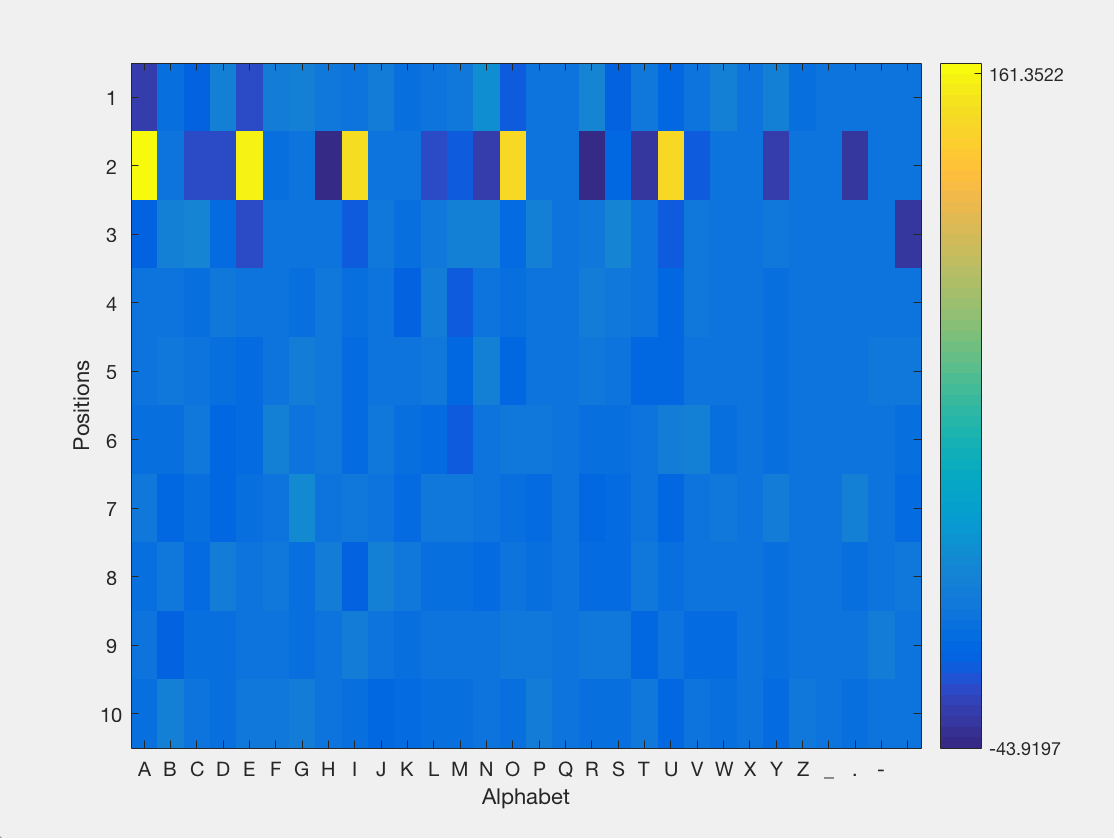
\includegraphics[scale = 0.7]{p3b3}\\
	As we can see, $\delta$ is very close to 0. In other words, we can conclude that the dataset is linear separable by the hyperplane. Also the test accuracy is perfect 1, which means our learning is successful. From the plot, there are five conspicuous yellow spots, which corresponds to Alphabet `A', `E', `I', `O' and `U' in the second position. Therefore, we can propose that it is positive when it's `A', `E', `I', `O' and `U' in the second position. 
	
	Next is my experiment time. I keep the $alphabet$ as original, but change $positions$ from $[1:10]$ to $[3:10]$. The results are different this time. \\
	\begin{center}
	delta = -2.4301e-12\\
	accuracyInTrain = 1\\
	accuracyInTest = 0.7234
	\end{center}
	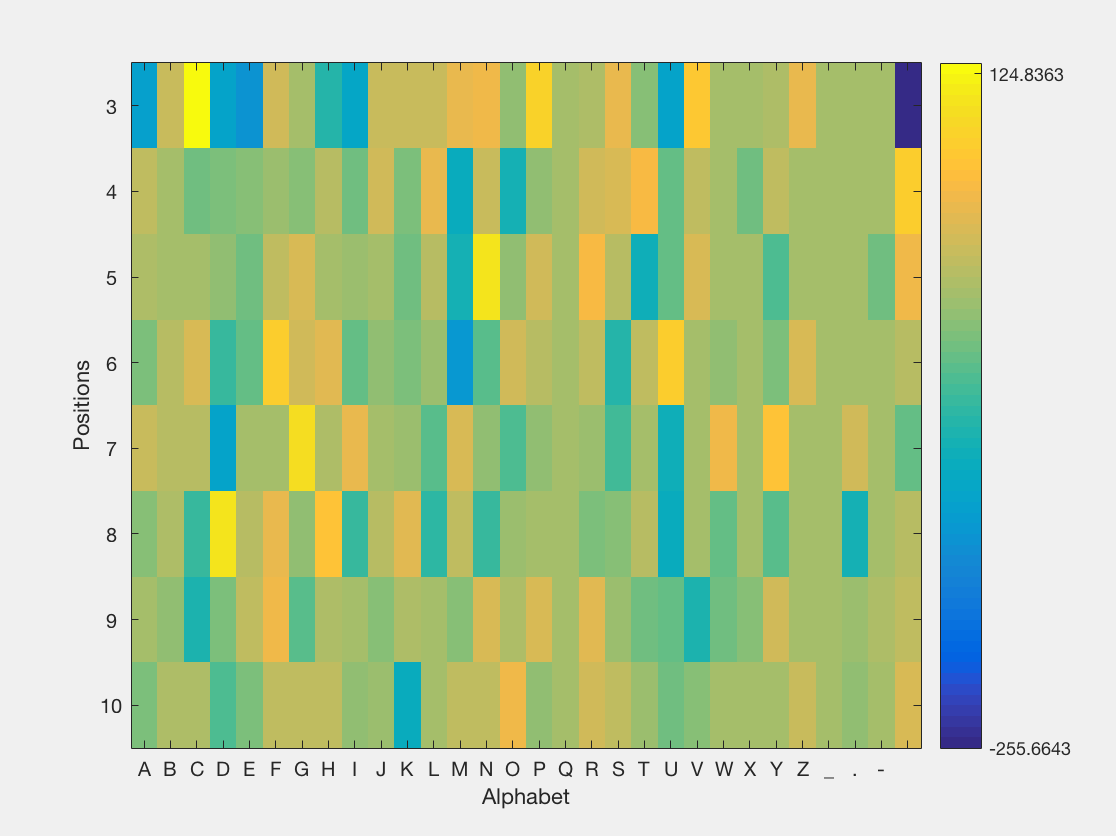
\includegraphics[scale = 0.7]{p3b3_changed}\\
	Similarly, $\delta$ is still close to 0, and the dataset can be separated by the result hyperplane. But the test accuracy is bad this time, around 0.7. The plot cannot clearly tell which weight is remarkably high or low compared to others. In this case, we cannot tell a general trend in order to conclude an accurate hypothesis.
	
	\item[b.4]
	The major difference between $findLinearThreshold$ and $findLinearDiscriminant$ is that we reduce the variable space from $[\vec{w},\theta,\delta]$ to $[\theta,\delta]$. A, b and c matrix will change correspondingly. Basically, we change A to a (m+1) by 2 matrix corresponding to m pairs of $[y_i, 1]$ and [0,1] in the end, and b to a (m+1) by 1 matrix with each row representing $1-y_i\vec{\omega}^T\vec{x}_i$. The cost vector now is simply $[0;1]$.\\
	A code snippet for $findLinearThreshold.m$ is given below.\\
	\noindent\rule[0.5ex]{\linewidth}{1pt}
	1.	function [theta,delta] = findLinearThreshold(data,w)\\
	2.	{\color{blue}\%\% setup linear program}\\
	3.	$[m, np1]$ = size(data);\\
	4.	n = np1-1;\\
	\newline
	5.	{\color{blue}\% write your code here}\\
	6.	x = data(:,1:n);\\
	7.	y = data(:,n+1);\\
	\newline
	8.	c = [0;1];\\
	\newline
	9.	A = ones(m+1,2);\\
	10.	for i=1:m\\
    	11.	\qquad A(i,1) = y(i);\\
	12.	end\\
	13.	A(m+1,1) = 0;\\
	\newline
	14.	b = zeros(m+1,1);\\
	15.	for i=1:m\\
    	16.	\qquad b(i) = 1-y(i)*dot(w,x(i,:));\\
	17.	end    \\
	18.	b(m+1) = 0;\\
	\newline
	19.	{\color{blue}\%\% solve the linear program}\\
	20.	{\color{blue}\%adjust for matlab input: A*x <= b}\\
	21.	$[t, z]$ = linprog(c, -A, -b);\\
	\newline
	22.	{\color{blue}\%\% obtain w,theta,delta from t vector}\\
	23.	theta = t(1);\\
	24.	delta = t(2);\\
	\newline
	25.	end\\
	\noindent\rule[0.5ex]{\linewidth}{1pt}
	
	The results are given below.
	\begin{center}
	\begin{tabular}{ | c | c | c | c | c | }
	\hline
	model & $\omega = [170, 294]^T$ & $\omega = [100, 300]^T$ & $\omega = [130, 100]^T$ & $\omega = [500, 100]^T$ \\
	\hline
	$\theta$ & -243.2630 & -218.9946 & -123.6116 & -344.3350\\
	\hline
	$\delta$ & -1.2506e-12 & -5.1159e-13 & 4.2917e-11& 92.9650\\
	\hline
	\end{tabular}
	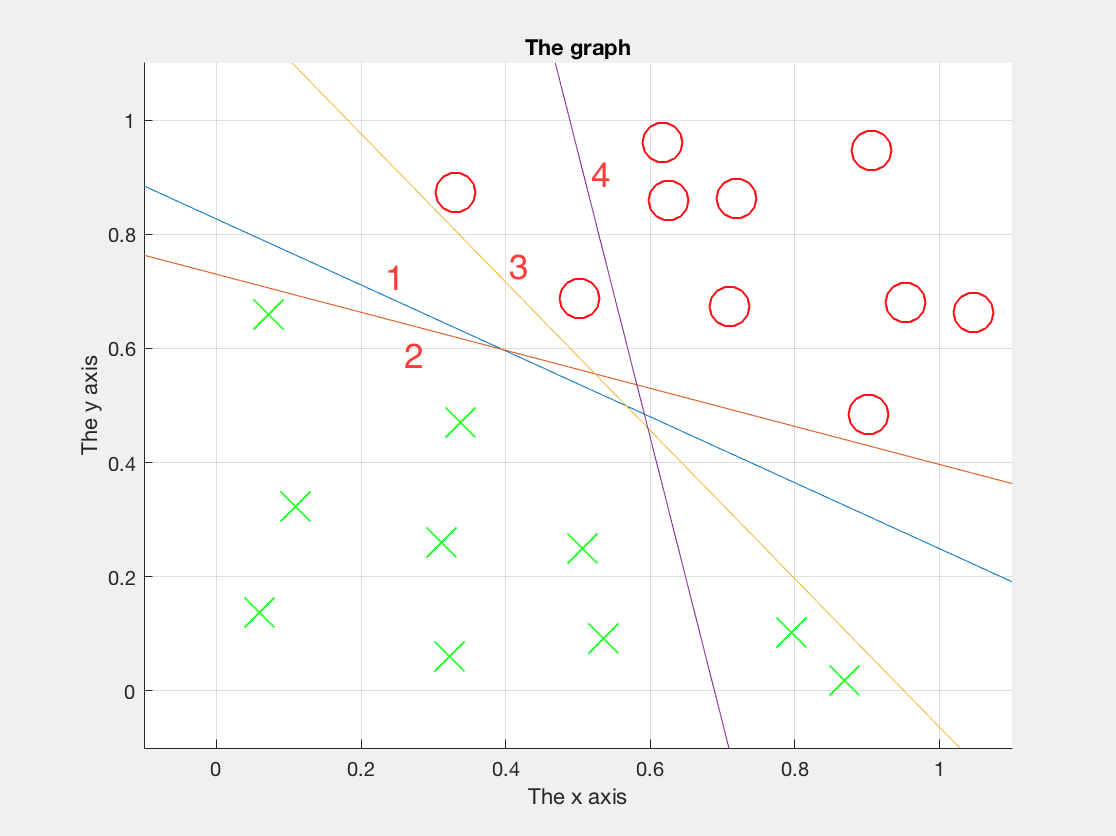
\includegraphics[scale = 0.65]{p3b4}\\
	\end{center}
	Line 1 is generated by the original problem with $\vec{\omega}$ also deducted by the algorithm $findLinearDiscriminant$. Other 3 lines are generated by specific weights. As we can see from the result, all but the 4th hyperplane can separate the dataset. It is consistent with $\delta$ value since it is really large at 92.9650 compared all others at around 0. For the three hyperplanes that separate the data, Line 1 does the job perfectly while Line 2 and 3 are quite close to either positive or negative data. Therefore, I would say hyperplane 1 is kind of better than others. But it really depends on the test data to tell which one is better. Also, based on the example, we cannot say the solution to linear program is unique because we have Line 2 and 3 here! Though both of them are not perfect separators with little margin, they still provide a new option for us. 

	\end{enumerate}

\end{enumerate}

\end{document}

